\chapter{Caractérisation et classification des procaryotes : de la cellule au génome}

Avant d'étudier la génomique des procaryotes, il convient de revenir sur ce qu'est un procaryote et comment le placer dans l'arbre du vivant. La classification du vivant est encore marquée de nombreux débats et donc elle est en perpétuel changement \cite{chun_integrating_2014}\cite{adl_revisions_2019}. De plus, il faut prendre en compte comment regrouper les individus en groupes (appelé taxon), c'est la taxonomie, mais aussi comment reconstruire les relations évolutives reliant les individus entre eux, c'est la systématique. Nous nous baserons sur la classification communément adoptée, c.-à-d., une division des êtres vivants en trois domaines : Bactéries, Archées et Eucaryotes\footnote{Dans cette vision de la classification, les virus ne sont pas intégrés, étant donné que leur appartenance au vivant est toujours débattue.}. Cette classification permet (dans de nombreux cas) de concilier une classification des espèces selon des critères phénotypiques et des critères génomiques.

\section{La classification des microbes : des critères phénotypiques à la biologie moléculaire}

Les premières classifications des microorganismes se sont appuyées sur des critères phénotypiques, c.-à-d., des caractéristiques observables. Bien que ces premières tentatives aient été limitées par la petite taille des organismes et les technologies, elles ont permis de distinguer plusieurs grands groupes.

Pour commencer, certains microorganismes sont pluricellulaires, comme les champignons du genre \textit{Penicillium}, tandis que d'autres, tels que la bactérie \textit{Escherichia coli}, ne sont constitués que d'une seule cellule et sont qualifiés d'unicellulaires. Dans la suite, nous nous concentrerons exclusivement sur les organismes unicellulaires\footnote{certains procaryotes montrent des formes de coopération et de différenciation cellulaire, suggérant une forme de multicellularité primitive. Cependant, elles ne sont pas multicellulaires au sens strict, car leurs cellules restent indépendantes sur le plan fonctionnel et structurel.}. 
La première distinction majeure qui a été établie pour diviser le vivant en deux grands domaines repose sur la présence ou l'absence de noyau. Le noyau est une structure interne de la cellule qui va contenir l'ensemble du matériel génétique. Les organismes (unicellulaires ou non) qui ont un noyau sont qualifiés d'eucaryotes. Pour ceux dont le matériel génétique est librement dispersé dans le cytoplasme, ils sont catégorisés dans le domaine des procaryotes. Ce sont ces derniers qui vont nous intéresser, et, sauf précision, ce qui sera dit s'appliquera à tous les procaryotes.

Le développement de la biologie moléculaire a permis d'affiner et de corriger les classifications précédentes en analysant la morphologie, la physiologie et la biochimie des cellules procaryotes, ainsi que les séquences d'ADN des génomes. C'est notamment en étudiant les gènes codant l'ARN 16S, qu'il a été mis en évidence que l'ensemble des procaryotes ne formait pas un groupe monophylétique, mais qu'ils étaient séparés en deux domaines, Bactérie et Archée\cite{woese_phylogenetic_1977}. Longtemps considéré comme des bactéries extrêmophiles, il est aujourd'hui clair que les Archées représentent un domaine à part entière avec toute sa singularité, comme la composition de leur membrane par exemple \cite{albers_archaeal_2011}. Malgré toute la fascination que nous pouvons avoir pour les archées, et que toutes les méthodes qui seront présentées peuvent s'appliquer aux espèces Archée, nous ne présenterons que très peu de résultats les concernant. C'est pourquoi dans la suite, même si nous parlerons de procaryote, nous considérerons plutôt le domaine des bactéries avec un prolongement possible aux archées.

\section{Taxonomie des procaryotes : un problème non résolu ?}

La classification des procaryotes et la définition d'espèce procaryote ne fait pas consensus dans la communauté des microbiologistes. Toutefois, les méthodes de classification se basent sur le même principe de relation entre les individus \cite{aldhebiani_species_2018}. Ces relations peuvent être soit phénétique, c.-à.-d, reposant sur la similarité d'un trait, sans s'intéresser au lien évolutif qui pourrait les relier, soit phylogénétique, c.-à.-d, reposant sur l'hérédité du caractère indépendamment de son état actuel.

Les premières tentatives de classification des bactéries reposaient sur des approches phénétiques, utilisant des critères basés sur les caractéristiques observables de ces organismes. Ces classifications s'appuyaient sur des caractères morphologiques, physiologiques et biochimiques.
D'un point de vue morphologique, les microbiologistes examinaient des paramètres tels que la taille des cellules, leur mode de croissance et leur capacité à former des agrégats spécifiques. La présence ou l'absence de structures spécialisées, telles que les flagelles, était également un critère de différenciation. 
Les caractéristiques physiologiques permettaient, quant à elles, de classer les bactéries selon leur mode de vie, leurs mécanismes métaboliques (anabolisme et catabolisme) et leurs réponses aux conditions environnementales.
L'étude de la composition cellulaire offrait par ailleurs de nouveaux outils pour affiner ces classifications sur le plan biochimique. Par exemple, la coloration de Gram, méthode emblématique, permet de différencier les bactéries en deux grands groupes : les Gram-positives, caractérisées par une paroi épaisse de peptidoglycane, et les Gram-négatives, qui présentent une paroi plus fine associée à une membrane externe lipidique.
Enfin, selon le contexte d’étude, d'autres critères peuvent être intégrés. Dans le domaine médical, la pathogénicité (capacité à induire une maladie) et le sérogroupage (basé sur la composition antigénique de la capsule bactérienne) sont particulièrement utilisés pour identifier et classifier les bactéries d'intérêt clinique.

Avec l'arrivée de la génomique, du séquençage et de la bioinformatique, ces classifications ont peu à peu laissé leur place à des classifications basées sur la phylogénie. Néanmoins, l'ADN a aussi été utilisé comme un critère phénétique définissant des critères biochimique comme similarité entre les souches. 
Dans ces critères, il y a d'abord le pourcentage de guanine-cytosine (GC) qui permet de différencier 2 souches appartenant à 2 genres différents si elles possèdent plus de 10 mol \%\footnote{1 équivalent molaire équivaut à 100 \% en mole, donc 10 \% en mole équivaut à 0,1 équivalent molaire.}, mais il faut noter qu'une composition en GC proche n'implique pas forcément que les souches soient proches. 
Une approche visant à définir formellement une espèce procaryote a été adoptée en 1987 par un comité d'expert \cite{moore_report_1987}. Il propose que des souches appartiennent à une même espèce si l'ADN s'hybride\footnote{Appariement de 2 brins d'ADN par complémentarité des bases} a plus de 70 \% et que le $\Delta T_m$\footnote{température à laquelle la moitié de l'ADN est dénaturés} diffère de 5 degrés ou moins.

Toutes ces approches ont permis de classer les procaryotes en taxon et dans la nomenclature de la taxonomie actuel, il reste des traces de ces méthodes. Elles sont d'ailleurs toujours utilisées et font partie des traits visible dans les classifications. Il faut d'ailleurs souligner qu'il n'est pas toujours possible d'obtenir des génomes de bonne qualité pour réaliser des phylogénies.

\section{Espèce procaryote : le génome complet et la phylogénie peuvent-ils trancher ?}

Les approches phénétiques présentées précédemment ont l'intérêt de s'appliquer directement au laboratoire et donc de regrouper et d'identifier les souches rapidement. Néanmoins, elles restent relativement approximatives et sont parfois coûteuses (en temps et en moyens). De plus, même si elles répondent aux problèmes de la taxonomie, et donc de ranger les bactéries dans des taxons, elles ne répondent pas à la question du lien entre les différents taxons et comment représenter ce lien, c.-à-d., à la question de la systématique.

Pour pallier les limites des approches précédentes, une nouvelle méthode a été développée et reste encore largement utilisée en routine aujourd'hui : la comparaison des souches à partir d'un gène marqueur. Il s'agit d'un gène présentant des variations spécifiques parmi les différentes souches d'intérêt, toutes dérivant d'une forme ancestrale commune ayant évolué différemment au fil du temps. Ainsi, le gène marqueur reflète à la fois la similarité entre les souches, permettant leur regroupement, et les événements dits de spéciation ayant conduit à leur séparation en espèces distinctes. On va privilégier l'utilisation de gènes hautement exprimés qui assurent une fonction essentielle à la vie de l'organisme : les gènes de ménage (\textit{house-keeping genes}). Un gène marqueur en particulier est utilisé : l'ADNr 16S, qui a la particularité d'être présent chez tous les procaryotes. En 2007, un arbre du vivant de toutes les espèces, a été reconstruit à partir d'un arbre d'ADNr 16S comprenant toutes les souches types séquencées d'espèces de bactéries et d'archées publiées jusqu'à la fin de l'année 2007 \cite{yarza_all-species_2008}. 
En allant encore plus loin, des analyses \textit{multilocus sequence analysis} MLSA ont été proposés \cite{glaeser_multilocus_2015}. Ces analyses prennent en compte plusieurs gènes marqueurs pour réaliser la taxonomie. L'utilisation de plusieurs gènes augmente le niveau d'information et réduit les biais. Toutefois, il n'y a pas de recommandation universelle pour réaliser l'analyse et chaque MLSA est réalisé en fonction des souches de départ. La sélection des gènes et leur nombre sont des paramètres qui ont un impact encore peu évalué sur la taxonomie. Il en va de même pour la taille des fragments considérés pour chaque gène, qui ne représente qu'une partie de la séquence du gène. Enfin, expérimentalement, il est souvent difficile, voire impossible, de concevoir des amorces facilitant l'amplification des gènes dans toutes les souches prises en compte. Malgré ces critiques, l'utilisation de gènes marqueurs est encore aujourd'hui utilisée, mais est peu à peu remplacée par des méthodes prenant en compte l'ensemble du génome.


Au début des années 2000 et avec les nombreux projets autour du séquençage et de l'analyse des génomes, comme le projet génome humain \cite{lander_initial_2001}, les technologies de séquençage sont de plus en plus précises et de moins en moins couteuse, amenant dans la génomique "moderne" : une augmentation exponentielle du nombre de séquences et des séquences plus longues et de meilleure qualité. C'est l'arrivée du \textit{Whole Genome Sequencing} (WGS) et de l'analyse de génomes complets de procaryote. En réalité, les premiers génomes complets ont été séquencés et assemblés il y a longtemps (1995), mais pour les utiliser en génomique comparée et en phylogénie, il fallait aussi que les technologies et les algorithmes bioinformatiques se développent à leur tour, c'est pourquoi les méthodes présentées précédemment étaient privilégiées.

Grâce aux nouvelles méthodes de génomique comparée, que nous présenterons dans le chapitre suivant, il est désormais possible de considérer le génome complet pour faire l'assignation taxonomique d'une bactérie. Une de ces approches est l'\textit{Average Nucleotide Identity} (ANI), qui rend compte de la similarité entre 2 séquences nucléotidiques. Le score d'ANI va d'ailleurs remplacer celui de l'hybridation, où un ANI inférieur 95 \% permet de différencier les espèces à la place d'une hybridation à 70 \% \cite{goris_dnadna_2007}. Plus récemment, le seuil de 95 \% a été confirmé par les auteurs de FastANI \cite{jain_high_2018}, utilisant plus de 90000 génomes. Ils ont montré l'existence d'un \textit{gap}, espace où l'ANI diminue fortement avant 95 \% (\autoref{fig:ANI_gap_sp}).


\begin{figure}[htbp]
    \centering
    % Première image
    \subfloat{%
        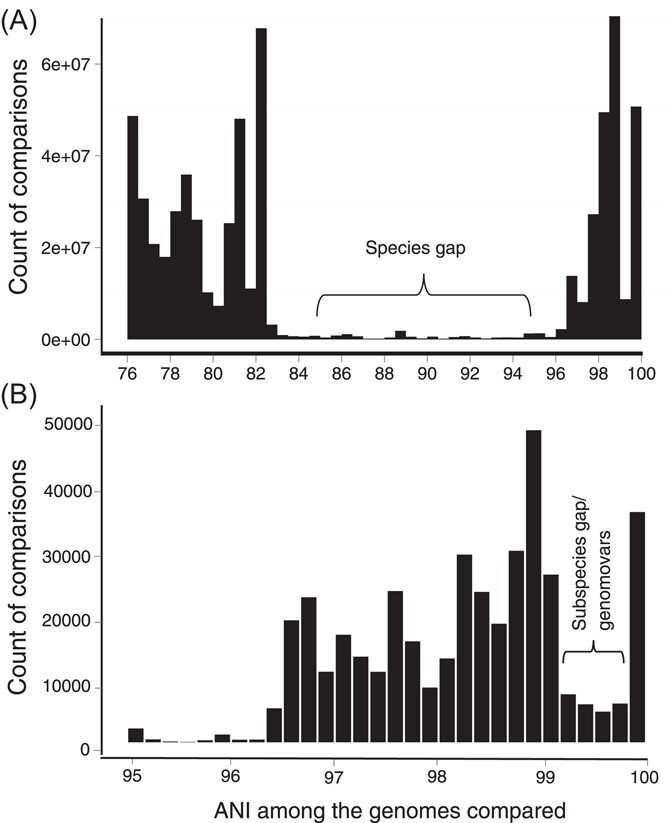
\includegraphics[width=0.48\textwidth]{images/ANI_gap.jpg}
    }
    \hfill % Espace flexible entre les deux images
    % Deuxième image
    \subfloat{%
        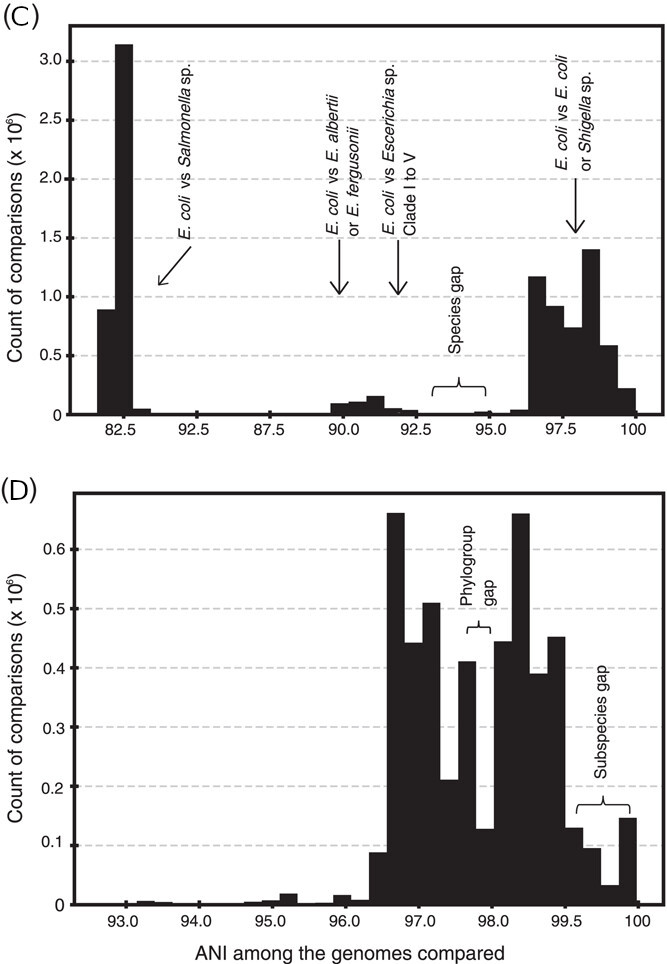
\includegraphics[width=0.48\textwidth]{images/ANI_sp.jpg}
    }
    \caption[Variation du score d'ANI au niveau de l'espèce]{Variation du score d'ANI au niveau de l'espèce. (A-B) Les histogrammes sont basés sur des comparaisons par paire effectuées avec FastANI. (A) Le Score d'ANI représenté au niveau de l'espèce se base sur les données de Jain \textit{et al}. On y retrouve un \textit{gap} entre 84 et 95 \% d'ANI. (B) Score d'ANI représenté au niveau intra-espèce sur les données de Rodrigues-R \textit{et al}. On retrouve un \textit{gap} entre 99,2 et 99,8 \% d'ANI. (C-D) Score d'ANI au niveau du groupe \textit{Escherichia coli}. Le nombre de génomes utilisés est le suivant : \textit{E. coli} : 2815 ; \textit{Salmonella enterica} : 1351 ; \textit{Escherichia fergusonii} : 57 ; \textit{Escherichia albertii} : 70 ; et \textit{Shigella flexneri} : 93 (tous les génomes complets disponibles au NCBI en juillet 2023). (C) Comparaison de l'ANI entre \textit{E.Coli} et d'autres espèces. Le seuil de 95 \% délimitant l'espèce est retrouvé. Un \textit{gap} à 97 \% existe entre \textit{E.coli} et \textit{Shigella flexneri} (une espèce d'\textit{E.Coli} particulière pour ces propriétés infectieuse). (D) Analyse de l'ANI au sein des génomes de \textit{E.Coli}. L'écart d'ANI de 99,5 \% est aussi prononcé, par rapport aux barres adjacentes, que l'écart d'ANI de 98 \%-97 \% qui correspond à l'écart entre les phylogroupes d'\textit{E. coli}, un groupe distinct et bien reconnu au sein d'\textit{E. coli}. Figures et légende adaptées de \cite{konstantinidis_sequence-discrete_2023}}
    \label{fig:ANI_gap_sp}
\end{figure}


Pourtant, la communauté n'est toujours pas arrivée à un consensus sur la classification des procaryotes en espèces et même sur l'existence d'espèces procaryotes. On peut d'abord critiquer l'approche et les résultats des études utilisant l'ANI, qui se limitent aux génomes de bonnes qualité et complets, ce qui \textit{de facto} limite le nombre de génomes et d'espèces potentielles pris en compte, tout en augmentant la redondance et limitant la diversité et la variabilité. De plus, la démarche apporte le biais d'utiliser une taxonomie déjà existante. Il faut aussi prendre en compte que la dynamique évolutive des procaryotes, que nous détaillerons dans le chapitre suivant (\autoref{sec:dyn_evo}), n'est pas linéaire et héréditaire, mais que les procaryotes sont capables de recevoir et d'échanger de l'ADN. C'est pourquoi des auteurs soutiennent une définition plus écologique de l'espèce bactérienne \cite{luo_genome_2011}, prenant en compte ces échanges agissant sur le \textit{fitness} des bactéries dans leur environnement.


On peut donc convenir qu'il n'est pas encore communément admis de parler d'espèce procaryote. Il existe toutefois des caractéristiques communes et spécifiques aux procaryotes ainsi que des traits propres à chaque taxon. De nombreuses méthodes et démarches scientifiques parviennent à construire une phylogénie des procaryotes, mais celle-ci doit être replacée dans son contexte d'étude pour prendre sens. Notamment en pangénomique, on étudie régulièrement le pangénome d'une espèce, il est donc nécessaire de se baser sur une classification des génomes en espèce. Dans le contexte de nos travaux, la similarité des séquences l'emporte comme critère de classification, nous utiliserons donc des génomes provenant de bases de données utilisant des critères comme l'ANI ou des gènes marqueurs pour construire des pangénomes.

%Enfin, avec l'explosion du nombre de séquences disponible, nous voyons l'émergence d'un paradoxe : de plus en plus de données sont disponibles, mais alors que l'on pensait pouvoir ranger les procaryotes dans des boites bien précises qui se verraient valider au cours du temps, une nouvelle exception vient renverser l'ordre actuel et la phylogénie doit être revue.
